\documentclass[12pt]{article}

\title{Research training portfolio}
\author{Wessel Stoop}

\usepackage{covington}
\usepackage{graphicx}
\usepackage{natbib}

\renewcommand{\familydefault}{\sfdefault}

\let\stdsection\section
\renewcommand\section{\newpage\stdsection}

\begin{document}
\maketitle

\begin{table}[h]
\begin{tabular}{ll}
Name&Wessel Stoop\\
Student numbers&s0808709 (Nijmegen), u1249664 (Tilburg)\\
Project&Fowlt, a context-based spelling checker\\
Supervisor&Antal van den Bosch\\
Period&September - December 2012\\
\end{tabular}
\end{table}

\section{Introduction}
Fowlt is the English version of the Dutch spelling checker Valkuil.net. Both Valkuil and Fowlt are unlike most well-known spell checkers (like the one in Microsoft Word): whereas these spelling checkers mostly try to find errors by comparing all words to a built-in dictionary and flag the word as an error if they can't find a match, Valkuil and Fowlt are 'context-based'. This entails that they also take into account the context, which is the words around every word. If, for a particular word, they expected another word based on the context, and the algorithm is really certain about it, it is flagged as an error. This means, for example, that Fowlt is able to replace the incorrect "there' in "there really nice people" into "they're" simply because "there" usually isn't followed by "really nice people", while "they're" is. 
\\\indent
To be able to make these kinds of correction suggestions, Fowlt makes use of language models. These models are created by giving lots of texts to the machine learning software TiMBL and WOPR. It's on the basis of these texts the model knows "there" mostly is not followed by "really nice people". However, this also means that if the context of a particular error is very different from what the model has seen in the training data, it won't be able to correct the error. This means users should be aware of the fact that, although Fowlt can recognize more kinds of errors than regular spell checkers, it might still miss a few. This is particularly true because Fowlt has been taught to only flag a word as an error if the algorithms are really sure about it.

\section{What I have done}
The best way to get a good overview of what I have done is probably to look at Fowlt's internal structure, so that's what I present in the next section. The first part of my internship basically consisted of adding the modules described below, one by one. To get a better idea of what parts took more time to 'get right', I also added a section about problems I encountered.

\subsection{Project structure}
Fowlt exist of multiple little spelling checkers, specialized in doing one thing. These spelling checkers are called 'modules'. Fowlt consists of four context-free modules (relatively similar to normal spelling checkers functionality) and, as I write this, sixteen context-based modules. This number will probably be different when you read this, though, as new context-based modules are created easily, and can be removed if it turns out they're not accurate enough.

\subsubsection{The processchain}
In Fowlt's main script, fowlt\_processchain.py, all modules are started up, and their outputs are collected. Making changes in this script (based on the one for Valkuil, written by Maarten van Gompel) to make sure the new English based modules worked correctly, is one of the main things I did during my internship.

\subsubsection{ErrorlistChecker (context-free)}
Martin Reynaert provided us with a large list of common typos and their corrections. This module, written by me, checks for every word in the input whether it's in the errorlist, and adds the correction when it is.

\subsubsection{LexiconChecker (context-free)}
Google provided us with an enormous list of word frequencies on the internet in 2008. The LexiconChecker checks for every word in the input whether there's a word on the frequencylist that is very similar to it, but much more frequent.

\subsubsection{RunonChecker (context-free)}
The RunonChecker also uses Google's list, but uses it to check if any spaces were forgotten in the input. This is done by looking whether splitting up long words produces two words which both are much more frequent that the original word.

\subsubsection{SplitChecker (context-free)}
The SplitChecker is the exact opposite of the RunonChecker: instead of looking whether any spaces are forgotten, it checks whether any spaces have to be added. This is done by looking whether each combination of two words produces a word which is much more frequent than the two original words.

\subsubsection{WOPRChecker (context-based)}
The WOPRChecker contacts WOPR, running on a server on localhost or elsewhere. It gives it the context of each word, but not the words themselves. If WOPR predicts another word with much certainty, this word is added as a correction.  

\subsubsection{The ConfusibleCheckers (context-based)}
The ConfusibleCheckers work similar to the WOPRChecker, with the only difference that they are trained on one specific language problem, instead of on language in general. As I write this, there are fifteen active ConfusibleCheckers, all focussing on their own expertise: lose-loose, it's-its, you're-your, than-then, who-which-that, whether-weather, effect-affect, lie-lay, they're-their-there, don't-doesn't,to-too-two, advice-advise, any-some, less-fewer, practice-practise and chose-choose.
\\\indent
A ConfusibleChecker trained on the difference between 'then' and 'than' for example filters out these two words and their contexts, sends these contexts to a Timblserver running somewhere. This Timblserver then says which of the two it would predict on the basis of the context. If this prediction is different from the actual word and the server is very sure about this, the word is flagged as an error. Training new ConfusibleModules has been a large part of my internship.

\subsection{Problems encountered}

\subsubsection{The original confusiblemodule could only handle two confusibles}
Most confusibles consist of two words only, but English has two that consist of three: they're-there-their and to-too-two. The original c-code could not handle confusibles with more than two words, so while the original plan was to either use Valkuil's c-code or rewrite it in Python, the quickest solution here was me diving into the c-code of my supervisor and add support for three.

\subsubsection{Problems with Ucto}
Although Ucto includes a configuration file for English, it didn't produce the correct output right out of the box. For example, for the It's-ItsModule to work, it is essential that "it's" is recognized as one word, which is not the case in original English configuration file. After a lot of tweaking of the regular expressions, I now have a tokenizer that produces output which can be used by all modules.

\subsubsection{The ConfusibleModules weren't good enough}
I didn't only train the ConfusibleModules, I also tested them with a program written by my supervisor. This program takes 10\% from the training data and saves it in a seperate file, trains TiMBL on the remaining 90\%, and then returns the percentage of correct predictions the resulting model can make about the 10\%. The results differed for the various confusibles, but the models were correct roughly 85-90\% of the time. This may seem a lot, but for a spellingchecker to be useful it's essential that a model can have an accuracy of over 99\%. Following the advice of my supervisor, I did two things to accomplish this: (1) I retrained TiMBL on the balanced training sets, which entails that there is an even amount of examples for each word the confusible consists of, and (2) I made the ConfusibleChecker only add a correction when it is very sure. Especially the latter solution increases the accuracy dramatically, but at the price of finding a lot less errors.

\subsection{Results}

\section{What I have learned}
Although had some experience with both programming and language technology, and even with some software co-developed by my supervisor, this internship turned out to be an adventure full of novelty: no single semester in my Radboud University career had such a high skills-acquired/day-ratio as this one. In the following sections, I give a non-exhaustive overview of what I learned while working on Fowlt.

\subsection{Working with Linux and SSH}
The novelty already started with something as non-trivial as the choice of operating system. As a Microsoft Windows user, I was surprised to find out all machine learning software I needed was developed and best used on Linux (see the next section). I only had a few hours of experience with Ubuntu, so I had to invest several hours into installing and getting more familiar with it. Ubuntu's GUI turned out to be almost identical to Windows', so most time went into learning the terminal commands. Unlike the commands for Windows' command prompt, Linux commands are essential for having full control. The first hours of the internship were therefore spent figuring out basic actions like \emph{ls} (showing folders and files in a directory) and \emph{mv} (renaming and moving files). This knowledge was also essential later, when I needed to control external servers over an SSH connection, as these Linux machines can be controlled with commands only. Here again, it took some time to figure out how to make the servers do what I wanted - transferring a python script from my machine to a server, for instance. Fortunately, working with Linux became routine quickly.

% Voordelen Linux?

\subsection{Working with machine learning software}
Fowlt uses the machine learning software TiMBL, TiMBLserver and WOPR. TiMBL consists of several memory-based learning algorithms, among which IB1-IG, an implementation of k-nearest neighbor classification with feature weighting suitable for symbolic feature spaces, and IGTree, a decision-tree approximation of IB1-IG. TiMBLserver adds server functionality to TiMBL. WOPR is a wrapper around the k-nearest neighbor classifier in TiMBL, offering word prediction and language modeling functionalities. Trained on a text corpus, WOPR can predict missing words, report perplexities at the word level and the text level, and generate spelling correction hypotheses. For Fowlt, only WOPR's spelling modus is used, of course.
\\\indent
Unfortunately, all three programs have very little documentation, and documentation that does exist often assumes background knowledge. With the help of my supervisor and Maarten van Gompel I learned how to (1) make language models by training the algorithms on large amounts of texts, (2) use these models to predict new words (and in my case, find spelling errors) and (3) test the model's accuracy. During my internship, I've repeated these three steps numerous times.
\\\indent
Besides TiMBL, TiMBLserver and WOPR, I also learned to use Ucto, software to tokenize texts so TiMBL and WOPR can handle them, and the PyNLPl Python library, which can read and create FoLiA-XML (among other things). FoLiA-XML is the XML-format used by Fowlt's output.

\subsection{Working with GitHub}
Working with multiple people on the same software can cause quite a lot of practical problems. Version control system Git solves these problems by keeping track of which version everyone of working on, providing tools to easily merge the work when done, and to remember older versions of the project, among other things. Although I had used Git for the latter function in personal hobby projects, I'd never worked together with other people on programming tasks. During this internship I learned (1) this can be done easily by using Git in combination with GitHub and (2) how to handle GitHub. GitHub is a website that offers open source projects a free, central and always reachable place for a Git repository, and also provides tools to look into this repo and its history online.

\subsection{Working with CLAM, setting up an NLP webservice}

\subsection{General}

% Python stuff
% C compilen

\section{Research paper}

\subsection*{Abstract}

For many confusibles, like "\emph{you're} versus \emph{your}", one option is much more frequent than the other. This poses a problem when one tries to create a context-sensitive memory-based confusible corrector, as having more data for one option will make it more likely that the confusible corrector will predict that option. In some cases this can be solved by balancing the training data so that it has exactly the same amount of examles for each option, but in other cases this means a very large part of the data have to be thrown away, making the corrector even worse. In this paper I investigate in which cases it is better to use a balanced training set, and in which cases it is better to train the modules on the larger, unbalanced set. I do this by building x confusible correctors and evaluating their results.

%hoeveel?

\subsection{Introduction}

This paper results from my attempts to solve a rather practical issue while building Fowlt, an online spell checker freely available on the internet. Fowlt, just like its Dutch equivalent Valkuil, is a context-sensitive spell checker. This context-sensitivity makes it possible to detect errors like the following:

\begin{examples}

\item There really nice people. \emph{Intended: they're.}
\item I'd like too see you two. \emph{Intended: to and too.}
\item I don't want to loose you. \emph{Intended: lose.}

\end{examples}

These errors, in which one word is confused with another (often homophone) word, are called \emph{confusible errors}. For the most common confusible errors, Fowlt contains a specialized modules. Unlike typos, confusible errors cannot be detected by simply looking at the text word for word, because the error is in the relation of a particular word with the other words in the sentence. Therefore, the confusible modules detect them by looking at the context of the word, and see if that differs from the contexts they have seen in the past for that word. If it, on the basis of the context, would predict another word in that position, and is really certain about it, it flags the word as an error. This means, for example, that Fowlt is able to replace the incorrect "there" in the last example into "they're", simply because "there" usually isn't followed by "really nice people", while "they're" is. \\\indent
This knowledge was not inserted manually, but was created with the help of Machine Learning software TiMBL. A more detailed account of its workings will be given in the next section. For now it is important to understand that TiMBL extracts this knowledge from large text corpora. From these corpora, all examples of the confusible have been extracted together with their content. The confusible corrector's results improve when TiMBL has seen more training material to base its decision on.\\\indent
Fowlt contains language models, and thus specialized confusible correctors, for the following confusibles (among others):

Dit is Fowlt. Dit is een confusible. Zo kan je ze herkennen. Dit hebben andere mensen gedaan. Dit zijn de confusibles waarnaar ik ga kijken. Dit zijn de verdelingen in mijn testset... kijk ze zijn scheef. Ik kan ze niet altijd weggooien, want dat wordt het nog erger. 

\subsection{Method}

% Hier moet ergens een beetje beschreven worden hoe zo'n Timblmodule werkt.

\subsubsection{Evaluation}

In this section, I describe the various evaluation measures I used. This is necessary because evaluation of spelling correctors has not been very uniform in the spelling checker literature so far; whereas various scholars only measured how many errors their algorithm can detect in an error list and called it accuracy (e.g. \citealp{agirre98, bm00, tm02,vandelden04}), others use or argue for the precision-recall terminology (\citealp{reynaert08,pz84}, although they use other terms for the two concepts) or argue against it \citep{sp02}.\\\indent

Although most of the evaluation measures used in the literature can be useful and informative, they only tell part of the story. I think it is important to recognize that spelling correction is a multi-step process, and each step comes with its own measures. When using a confusible module as part of a spelling corrector, there are three steps: word prediction, error detection and error correction. I'll go through these steps and their evaluation measures one by one.

\paragraph{Word prediction}

\begin{itemize}
\item Prediction accuracy. Although word prediction may be the most complicated part of the confusible module, its evaluation is actually the simplest. Calculating prediction accuracy entails removing all confusibles from a text, and see in how many of the cases the language model can correctly predict which word was removed. This percentage can be increased by only counting predictions that are above a certain threshold. Results with multiple thresholds (i.e. to what extent does the prediction accuracy improve if the threshold is raised?) can be visualized with a graph, as shown in the result section.
\end{itemize}

\paragraph{Error detection}

\begin{itemize}
\item The confusion matrix. From this step onwards, we concentrate on spelling errors. This means that our input no longer is errorless text, like in the previous step. We also interpret the results of the prediction differently now: whereas incorrectly predicted words were considered errors of the system in the previous task, lowering the accuracy, they will now be considered corrections. This means that the system can do two things right (correct incorrect words in the text and don't correct correct words), and two things wrong (correct correct words and don't correct incorrect words). This can be summarized in a confusion matrix (taken from \citet{fawcett04}):

\begin{figure}[htb]
\centering
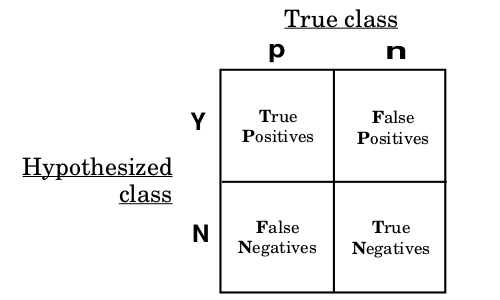
\includegraphics[width=0.8\textwidth]{confusion_matrix.png}
\caption{The confusion matrix}
\label{fig:confusion}
\end{figure}

When reporting the results of a confusible module, the names of the various cells will be replaced by numbers. These numbers are the data needed to calculate various evaluation measures, like the three below. Beside these evaluation measures, I will always give the confusion matrix itself, so readers can calculate other measures if desired.

\item Detection accuracy. Detection accuracy only indicates how many mistakes the confusible detector makes, not what kind of mistakes. It can be calculated with the following formula:

%formula

It is similar to prediction accuracy in that it indicates how well the sytem does in general, but keep in mind that prediction and detection accuracy measure two completely different concepts. Although a system with a good prediction accuracy is very likely to also have a good detection accuracy, it might be possible that a system very good at predicting confusibles in errorless texts behaves differently in texts that do contain errors.
 
\item Detection recall.
\item Detection precision.
\end{itemize}

\paragraph{Error correction}

\begin{itemize}
\item Confusion matrix.
\item Detection accuracy.
\item Detection recall.
\item Detection precision.
\end{itemize}

\paragraph{Problems with precision and recall.} Some text.

Waarom geen AUC?

\subsection{Results}

\subsection{Conclusion}

\section{General conclusion}

\begin{thebibliography}{99}

\bibitem[Agirre et al., 1998]{agirre98}
Agirre et al., 1998
\bibitem[Brill \& Moore, 2000]{bm00}
Brill \& Moore, 1998
\bibitem[Van Delden et al., 2004]{vandelden04}
Van Delden et al, 2004.
\bibitem[Fawcett, 2004]{fawcett04}
Fawcett, 2004.
\bibitem[Pollock \& Zamora, 1984]{pz84}
Pollock \& Zamora, 1984
\bibitem[Reynaert, 2008]{reynaert08}
Reyneart, 2008.
\bibitem[Starlander \& Popescu-Belis, 2002]{sp02}
Starlander \& Popescu-Belis, 2002
\bibitem[Toutanova \& Moore, 2002]{tm02}
Toutanova \& Moore, 2002.

\end{thebibliography}

% Ene paper Antal
% roc101

\end{document}
